% !TEX root = ../Thesis.tex

\chapter{Methodology}\
\label{ch:methodology}

\begin{figure}[h] %h can be omitted for better page layout
  \begin{center}
    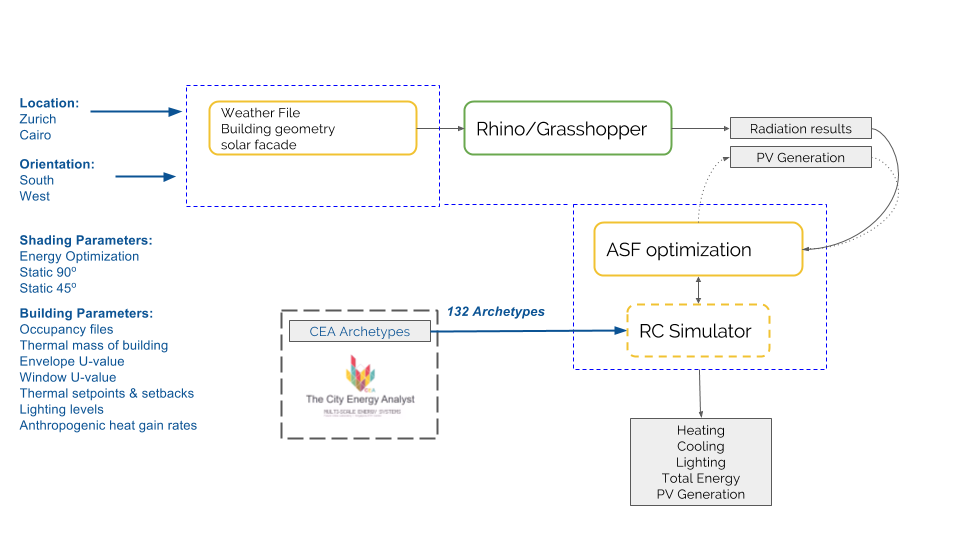
\includegraphics[width=\textwidth, trim= 0cm 0cm 0cm 0cm,clip]{methodology.png}
    \caption{ASF simulation workflow at the time of writing}
    \label{fig: methodoloy}
  \end{center} 
\end{figure}

Code for a basic 1R1C model was written. Building Geometry was kept consistent with Ladybug ASF tests. 1R1C was compared to free-running 3R1C without internal gains, then with solar and occupancy gains. Same again with the 5R1C, which was coded by PJ using the model in ISO13790 Annex C. This model was integrated with code from Mauro Luzzatto's ongoing thesis project, \textit{Numerical Analysis of the Adaptive Solar Facade}, producing a building simulation tool for a single zone with the ASF.\par


Building properties first set in python, links with grasshopper to run simulation (soon to be replaced) which takes 50 hours, back to python to run PV, from then on simulations (with optimization) take less than a minute per building.\par
Simulation parameters: 
CEA database provides 15 archetypes of which 11 are used: 
Multi-residential, single- residential, hotel, office, retail, foodstore, restaurant, industrial, school, hospital, gym.
For each archetype:

\begin{itemize}
 \item Building age: building properties for six distinct periods are provided: 1920, 1920-1970, 1970-1980, 1980-2005, 2005-2020, 2020-2030. In addition, two sets of properties are defined: one for new construction and another for renovation. It would be possibile to first study new buildings, and later expand to older buildings
 \item Go through the other CEA Archetypes
 \item Schedules: Probability of occupancy, lighting, and electrical appliances on given weekdays and weekends need to figure out how to use them
 \item Room geometry parameters: different glazing ratios/room dimensions --- check limits in ISO standard [not done because of huge computational time]
 \item Weather file and orientation: [Zurich S, Zurich W, Cairo S, Cairo W] - with ASF and without ASF
 \item Systems analysis: analyse the effectiveness of different heating and cooling systems coupled with the ASF [should be a separate study]
\end{itemize}

